\section{Use cases}
Now we are going to depict goals of users which the application will make achievable.
Figure 2.1 contains a use case diagram of the application.
A use case styled with a bold border indicates that it groups together more use cases and will be further expanded later.
All use cases will be structurally described by independent use case scenarios.

\begin{figure}[h]
    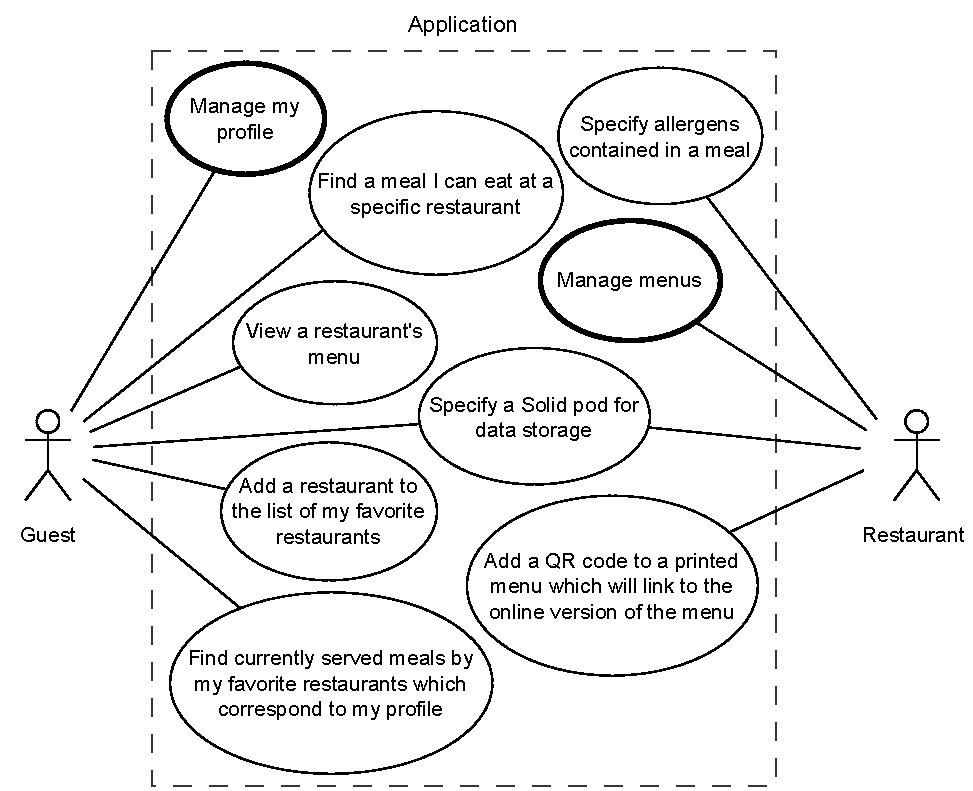
\includegraphics[width=\linewidth]{master-thesis/img/application_use_cases}
    \caption{The application's use case diagram.}
\end{figure}

% Add top padding for scenario tables
\def\arraystretch{1.5}

\subsection{Guest use cases}

\begin{center}
\begin{tabular}{| l | p{10.75cm} | }
  \hline
  Actor & Restaurant \\
  \hline
  Scenario & 
\begin{minipage}[t]{\linewidth}
    \begin{enumerate}[leftmargin=*,nosep,before=\vspace{-0.575\baselineskip},after=\strut]
    \item lorem ipsum
    \item lorem ipsum
\end{enumerate}
\end{minipage}
  \\
  \hline
  Alternatives &     
    \begin{minipage}[t]{\linewidth}
    \begin{description}[nosep,after=\strut]
        \item [A1] First
        \item [A2] Second
    \end{description}
    \end{minipage}
  \\
  \hline 
\end{tabular}
\end{center}

\begin{center}
\begin{tabular}{| l | p{10.75cm} | }
  \hline
  Actor & Restaurant \\
  \hline
  Scenario & 
\begin{minipage}[t]{\linewidth}
    \begin{enumerate}[leftmargin=*,nosep,before=\vspace{-0.575\baselineskip},after=\strut]
    \item lorem ipsum
    \item lorem ipsum
\end{enumerate}
\end{minipage}
  \\
  \hline
  Alternatives &     
    \begin{minipage}[t]{\linewidth}
    \begin{description}[nosep,after=\strut]
        \item [A1] First
        \item [A2] Second
    \end{description}
    \end{minipage}
  \\
  \hline 
\end{tabular}
\end{center}

\begin{center}
\begin{tabular}{| l | p{10.75cm} | }
  \hline
  Actor & Restaurant \\
  \hline
  Scenario & 
\begin{minipage}[t]{\linewidth}
    \begin{enumerate}[leftmargin=*,nosep,before=\vspace{-0.575\baselineskip},after=\strut]
    \item lorem ipsum
    \item lorem ipsum
\end{enumerate}
\end{minipage}
  \\
  \hline
  Alternatives &     
    \begin{minipage}[t]{\linewidth}
    \begin{description}[nosep,after=\strut]
        \item [A1] First
        \item [A2] Second
    \end{description}
    \end{minipage}
  \\
  \hline 
\end{tabular}
\end{center}

\subsection{Restaurant use cases}



\subsection{Mutual use cases}

